\documentclass{article}
\usepackage[utf8]{inputenc}

\usepackage{geometry}
\usepackage[danish]{babel}
 \geometry{
 a4paper,
 total={140mm,227mm},
 left=35mm,
 top=35mm,
 }
 

\usepackage{float}
\usepackage{graphicx}
\usepackage{epstopdf}
\usepackage{amsmath}
\usepackage{amssymb}
\usepackage{mathtools} 
\usepackage{bm}
\usepackage{color}

\usepackage{hyperref}
\hypersetup{
    colorlinks=true,
    linkcolor=black,   
    urlcolor=black,
    filecolor=black,
} 
\urlstyle{same}

\usepackage{ dsfont }
\numberwithin{equation}{section}

\usepackage{xcolor}
\usepackage{mdframed}

\input{tikz.tex} % sætter tikz op til at lave tableauer 

\newlength\tindent
\setlength{\tindent}{\parindent}
\setlength{\parindent}{0pt}
\renewcommand{\indent}{\hspace*{\tindent}}

\title{01017 Diskret Matematik A3}
\author{s144107 Roar Nind Steffensen \\ s144063 Magnus Middelboe Søborg-Madsen}
\date{\today}

\begin{document}

\maketitle

\section{Bridge}

\subsection*{(a) Sætning 1.4}

Vi skal vise at $2^n = \sum_{k=0}^{n} {n \choose k}$.\\
\\
Vi benytter sætning 1.4:

\begin{mdframed}[backgroundcolor=gray!5]
\begin{equation}
    (X+Y)^n = \sum_{k=0}^{n} {n \choose k} \cdot X^{n-k} \cdot Y^{k}
\end{equation}
\end{mdframed}
\vspace{0.5 cm}

Vi indsætter $X=Y=1$:
\begin{equation}
    (1+1)^n = \sum_{k=0}^{n} {n \choose k} \cdot 1^{n-k} \cdot 1^{k}
\end{equation}

For alle $c \in \mathbb{Z}$ er $1^c$ = $1$, så $1^{n-k}=1$ og $1^{k}=1$. Dvs.
$1^{n-k} \cdot 1^{k} = 1$. Vi har da

\begin{equation}
    (1+1)^n = \sum_{k=0}^{n} {n \choose k} \cdot 1
\end{equation}

\begin{equation}
 2^n = \sum_{k=0}^{n} {n \choose k}
\end{equation}

som ønsket.

\subsection*{(b) Bridgehænder}
Vi vil finde antallet af mulige bridgehænder. Der er $n=52$ kort. Vi skal vælge $k=13$ kort. Rækkefølgen er ligegyldig. Antallet af mulige bridgehænder er da givet ved binomialkoefficienten, der udregnes via sætning 1.3:

\begin{equation}
    N_{\text{total}} = {n \choose k} = {52 \choose 13} = \frac{52!}{(52-13)! \cdot 13!} = \frac{52!}{39! \cdot 13!} = 635013559600 \approx 6.35 \cdot 10^{11}
\end{equation}

\subsection*{(c) 4-3-3-3 fordeling}

Vi vil nu finde antallet af bridgehænder med en 4-3-3-3 fordeling.\\
\\
Vi bruger igen binomialkoefficienten givet ved sætning 1.3, fordi rækkefølgen er ligegyldig. Hvis spilleren trækker hjerter 1 og så hjerter 2, er det det samme som at trække hjerter 2 og så hjerter 1.\\
\\
Antag at vi starter med et at trække et kort af kuløren \textcolor{red}{\textbf{hjerter}}. Der er 13 kort af denne kulør, og vi skal trække 4 af dem.  Derefter skal vi trække 3 af de 13 \textbf{spar}. Så 3 af de 13 \textcolor{orange}{\textbf{ruder}}. Endeligt 3 af de 13 \textcolor{blue}{\textbf{klør}}.
\\
\\
Dvs. hvis vi skal 4 hjerter kort, og 3 af de resterende kulører, er der umiddelbart

\begin{equation}
     N_{\text{hjerter start}} = \textcolor{red}{{13 \choose 4}}  \cdot {13 \choose 3} \cdot  \textcolor{orange}{{13 \choose 3}} \cdot  \textcolor{blue}{{13 \choose 3}} 
\end{equation}

forskellige hænder af \textcolor{red}{4}-\textcolor{black}{3}-\textcolor{blue}{3}-\textcolor{orange}{3} fordeling med 4 hjerter kort. Men! Der er 4 forskellige kulører, der kan være den "store" del af hånden (de 4 kort). Så antallet af mulige 4-3-3-3 bridgehænder er givet ved

\begin{equation}
     N_{\text{4-3-3-3}} = {13 \choose 4}  \cdot {13 \choose 3}^3 \cdot 4 = \frac{13!}{(13-4)! \cdot 4!} \cdot \left( \frac{13!}{(13-3)! \cdot 3!} \right)^3 \cdot 4
\end{equation}

\begin{equation}
     N_{\text{4-3-3-3}} = \frac{13!}{9! \cdot 4!} \cdot \left( \frac{13!}{10! \cdot 3!} \right)^3 \cdot 4 = \frac{13!^4 \cdot 4}{9! \cdot 4! \cdot 10!^3 \cdot 3!^3} = 66905856160 \approx 6.69 \cdot 10^{10}
\end{equation}

Andelen af bridgehænderne, der er 4-3-3-3 hænder, er da

\begin{equation}
    \frac{N_{\text{4-3-3-3}}}{N_{\text{total}}} \approx \frac{6.69 \cdot 10^{10}}{6.35 \cdot 10^{10}} \approx 0.105 = 10.5 \, \%
\end{equation}
\section{Rekursion}

\subsection*{(a) $f(n)$}

Vi vil vise, at antallet af ord $f(n)$ med længden $n$ bogstaver, som følger de givne regler i opgavesættet, er givet ved:
\[ f(n) = \begin{cases} 
      0 & n < 0 \\
      1 & n = 0 \\
      2 f(n-1) + 2 f(n-2) & n > 0
   \end{cases}
\]
\\

Vi betragter først basistilfældene $n<0$ og $n=0$.\\
\\
$n<0$: Det er ikke muligt at lave ord med et negativt antal bogstaver, så $f(n)=0$ for $n<0$.\\
$n=0$: Der er kun én måde, vi kan lave et ord med 0 bogstaver, nemlig ved ikke at bruge nogen bogstaver. Så $f(0)=0$.\\
\\
$n>0$: Vi betragter et vilkårligt legalt ord med $n>0$ bogstaver, der ender på $a$ eller $b$. Vi skriver det som
\begin{equation}
    [\quad]_0 \, ... \, [\quad]_{n-2} \, [\quad]_{n-1} \, [a/b]_n, 
\end{equation}

hvor kantede parenteser repræsenterer et bogstav, og sænket skrift repræsenterer bogstavet indeks. Det sidste bogstav læses "$a$ eller $b$". Vi forestiller os, at vi fjerner det $n$'te bogstav. Er ordet med $(n-1)$ bogstaver et legalt ord?\\
\\
\textcolor{red}{\textbf{Case 1}} og \textcolor{blue}{\textbf{Case 2}}: Hvis det $(n-1)$'te bogstav er $a$ eller $b$, og alle forrige bogstaver overholder reglerne, er det $(n-1)$'te ord legalt. Efter at have fjernet det $n$'te $a$ (eller $b$), er vi tilbage til start: vi har et legalt ord med $(n-1)$ bogstaver, der slutter med $a$ eller $b$.\\
\\
\textcolor{orange}{\textbf{Case 3}} og \textcolor{black}{\textbf{Case 4}}: Hvis det $(n-1)$'te bogstav er et $c$, er ordet med $(n-1)$ bogstaver ikke legalt. Men hvis det $(n-2)$'te bogstav er et $a$ eller $b$, og alle de forrige bogstaver overholder reglerne, er ordet med $(n-2)$ bogstaver et legalt ord. Efter at have fjernet det $n$'te $a$ (eller $b$) og det $(n-1)$'te $c$, er vi tilbage til start: vi har et legalt ord med $(n-2)$ bogstaver, der slutter med $a$ eller $b$.

\begin{figure}[H]
\centering
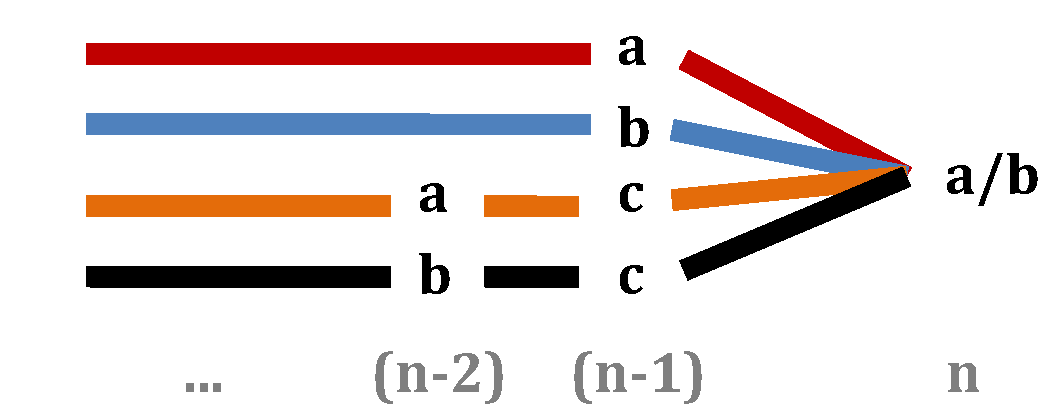
\includegraphics[width=0.7\textwidth]{Opg2/fig/2a.pdf}
\caption{Visualisering af legale ord. Rækkefølgen af bogstaver er $(n-2) \quad (n-1) \quad n$.}
\label{fig:2a}
\end{figure}

Der findes således \textcolor{red}{$f(n-1)$} legale ord, der slutter med $a$ og er ét bogstav kortere end $[\quad]_0 \, ... \, [\quad]_{n-2} \, [\quad]_{n-1} \, [a/b]_n$. Der findes også \textcolor{blue}{$f(n-1)$} legale ord, der slutter med $b$ og er ét bogstav kortere.\\
\\
Der findes \textcolor{orange}{$f(n-2)$}+\textcolor{black}{$f(n-2)$} legale ord, der er to bogstavere kortere end \\
$[\quad]_0 \, ... \, [\quad]_{n-2} \, [\quad]_{n-1} \, [a/b]_n$.\\

Så hvor mange legale ord kan vi skrive med $n$ bogstaver?
\begin{equation}
f(n) = \textcolor{red}{f(n-1)} + \textcolor{blue}{f(n-1)} + \textcolor{orange}{f(n-2)}  + \textcolor{black}{f(n-2)} = 2 f(n-1) + 2 f(n-2)
\end{equation}

som ønsket.

\subsection*{(b) $f(4)$}
$f(-1)=0$ og $f(0)=1$ ifølge definitionen. Vi beregner $f(n)$ og $n!$ for udvalgte værdier. $f(n)$ beregnes ved 2 gange summen af de to forrige elementer:
\begin{equation}
f(n) = 2 f(n-1) + 2 f(n-2) = 2 \left( f(n-1) + f(n-2) \right)
\end{equation}

\renewcommand{\arraystretch}{1.3}
\begin{table}[H]
\begin{center}
    \begin{tabular}{ccccccccc}
    \hline
    $n$    & $-$1 & 0 & 1 & 2 & 3  & 4  & 5   & 6   \\ \hline
    $f(n)$ & 0  & 1 & 2 & 6 & 16 & 44 & 120 & 328 \\ \hline
    $n!$   &   & 1 & 1 & 2 & 6  & 24 & 120 & 720 \\ \hline
    \end{tabular}
    \vspace{-0.5cm}
    \caption{Udvalgte værdier af $f(n)$ og $n!$.}
    \label{tab:2b}
    \end{center}
\end{table}
\renewcommand{\arraystretch}{1.0}

Dvs. $f(4)=44$.

\subsection*{(c) $f(n) < n!$}
Det ses i tabel \ref{tab:2b} at $f(n) < n!$ for $n=6$. Så der findes et $n \in \mathbb{N}$ således at $f(n) < n!$.\\
\\
Man kan undersøge højere værdier for $n$. Det viser sig at for alle $n \geq 6$ er $n! > f(n)$ da $\frac{f(n+1)}{f(n)}$ konvergerer mod $2.73205$ (undersøgt med WolframAlpha) for $n \rightarrow \infty$, mens $\frac{(n+1)!}{n!}$ divergerer for $n \rightarrow \infty$. Opgaven spurgte dog kun om der findes ét $n$.
\section{Induktion}
%Skabelon fra lecture slides:
%\begin{figure}[H]
%\centering
%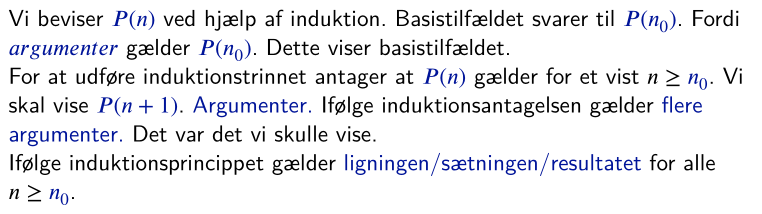
\includegraphics[width=1.0\textwidth]{Opg3/fig/3a_skabelon.png}
%\caption{Visualisering af legale ord. Rækkefølgen %af bogstaver er $(n-2) \quad (n-1) \quad n$.}
%\label{fig:2a}
%\end{figure}

Vi betragter for $n \in \mathbb{N}$ funktionen $f(n)$ defineret ved 

\begin{equation}
\label{eq:def}
f(n) = \sum_{k=0}^{n} 2^k
\end{equation}

Vi vil bevise ved induktion at der for alle $n \in \mathbb{N}$ gælder 

\begin{equation}
    f(n) = 2^{n+1} -1
\end{equation}

\textbf{Basistilfælde}\\
Basistilfældet svarer for $n_0 = 0$ til
\begin{equation}
    f(0)= 2^{0+1} -1=2-1 = 1
\end{equation}


Vi indsætter $n=0$ i definitionen \ref{eq:def}:
\begin{equation}
f(0) = \sum_{k=0}^{0} 2^k = 2^0 = 1
\end{equation}

Definitionen og induktionsantagelsen giver samme resultat. Dette viser basistilfældet.\\
\\
\textbf{Induktionstrin}\\
For at udføre induktionstrinnet antager vi at $f(n) = 2^{n+1} -1$ gælder for et $n \geq n_0$. Vi skal vise at $f(n+1)=2^{(n+1)+1} -1 = 2^{n+2} -1$. Dvs. hvis formlen virker for $n$, skal den også virke for $n+1$.\\
\\
Vi beregner $f(n+1)$ via definitionen, og tager det sidste led ud af summen:
\begin{equation}
f(n+1)= \sum_{k=0}^{n+1} 2^k = 2^{n+1} + \textcolor{red}{\sum_{k=0}^{n} 2^k}
\end{equation}

Vi anvender induktionsantagelsen, og substituerer:

\begin{equation}
f(n+1) = 2^{n+1} + \textcolor{red}{2^{n+1}-1}
\end{equation}

Vi simplificerer ved brug af eksponentregler:

\begin{equation}
f(n+1) = 2 \cdot 2^{n+1} -1 = 2^{n+2} -1
\end{equation}

Dvs. ifølge induktionsagelsen gælder $f(n+1) = 2^{n+2} -1$. Det var det, vi skulle vise. \\
\\
\textbf{Konklusion}\\
Ifølge induktionsprincippet gælder da $f(n) = 2^{n+1} -1$ for alle $n \geq n_0$. Da $n_0 = 0$, gælder formlen således for alle $n \in \mathbb{N}$. 



\end{document}
